\documentclass[10pt]{beamer}

\usepackage{xeCJK}

\usepackage[T1]{fontenc}

\usepackage[utf8]{inputenc}

\usetheme{metropolis}
\usepackage{appendixnumberbeamer}

\usepackage{booktabs}
\usepackage[scale=2]{ccicons}

\usepackage{pgfplots}

\usepackage{xspace}

\usepackage{listings}

\lstset{
	basicstyle=\ttfamily,
	escapeinside=||
}

\usepackage{graphicx}

\newcommand{\emptyline}{\vspace{\baselineskip}}

\usepackage{ulem}


\title{程序设计教程}
\subtitle{环境搭建和C语言入门}
\date{2019-10-25}
\author{唐瑞泽}
\institute{tangruize@smail.nju.edu.cn}

\begin{document}
	
\maketitle

\begin{frame}{目录}
	\setbeamertemplate{section in toc}[sections numbered]
	\tableofcontents[hideallsubsections]
\end{frame}

\section{环境搭建}

\begin{frame}[fragile]{第一个程序}
\begin{columns}[T,onlytextwidth]
\column{0.50\textwidth}
\begin{block}{源代码}
\small\begin{lstlisting}[language=c]
#include <stdio.h>
int main() {
    printf("Hello, world!\n");
}
\end{lstlisting}
\end{block}

\column{0.05\textwidth}
\begin{block}{}\end{block}
\begin{block}{->}\end{block}
\begin{block}{}\end{block}

\column{0.30\textwidth}
\begin{block}{执行结果}
\small\begin{lstlisting}
Hello, world!
\end{lstlisting}
\end{block}
\end{columns}

\begin{itemize}[<+- | alert@+>]
\item C源代码是如何变成 exe 文件的呢?
\item 编译
\end{itemize}
\end{frame}

\begin{frame}[fragile]{如何编译C源代码?}
\begin{itemize}[<+- | alert@+>]
\item 需要一个编译器
\item 常见的编译器: GCC, CLANG, MSVC
\item 以GCC为例, 编译并执行main.c
\begin{verbatim}
  gcc main.c -o main
  ./main
\end{verbatim}
\item 代码用什么修改? VIM? EMACS?
\item 改了代码再编译呢? 重新敲一遍? 写个脚本或Makefile?
\item 出BUG了,怎么调试呢? 听说可以用GDB?
\item \sout{可是vim, gcc, make, gdb我都不会啊}
\item 你需要一个集成开发环境(IDE)
\end{itemize}
\end{frame}

\begin{frame}[fragile]{集成开发环境}
VS和CLion都很优秀, 这里有安装教程:
\href{http://problemoverflow.top/c/0.%E5%BC%80%E5%8F%91%E7%8E%AF%E5%A2%83%E6%90%AD%E5%BB%BA/0.0.Microsoft_Visual_Studio.html}{VS},
\href{http://problemoverflow.top/c/0.%E5%BC%80%E5%8F%91%E7%8E%AF%E5%A2%83%E6%90%AD%E5%BB%BA/0.1.CLion.html}{CLion}

CLion相比于VS有许多\href{http://problemoverflow.top/index.php?qa=33&qa_1=%E6%89%80%E4%BB%A5%E5%88%B0%E5%BA%95%E7%94%A8%E4%BB%80%E4%B9%88-ide-%E5%86%99-oj%EF%BC%9F&show=36#a36}{优点}
\begin{itemize}
\item 使用跨平台的CMAKE管理工程
\item 编辑器提示更智能
\item 可高度定制等
\end{itemize}
如果还没有安装CLion, 请下载: \href{https://www.jetbrains.com/clion/download}{CLion}, \href{https://nchc.dl.sourceforge.net/project/mingw-w64/Toolchains%20targetting%20Win64/Personal%20Builds/mingw-builds/8.1.0/threads-posix/seh/x86_64-8.1.0-release-posix-seh-rt_v6-rev0.7z}{MinGW}
\end{frame}

\begin{frame}[fragile]{CLion快速配置}
\href{https://nchc.dl.sourceforge.net/project/mingw-w64/Toolchains%20targetting%20Win64/Personal%20Builds/mingw-builds/8.1.0/threads-posix/seh/x86_64-8.1.0-release-posix-seh-rt_v6-rev0.7z}{MinGW} (提供make, gcc, g++, gdb):

解压缩 \href{https://nchc.dl.sourceforge.net/project/mingw-w64/Toolchains%20targetting%20Win64/Personal%20Builds/mingw-builds/8.1.0/threads-posix/seh/x86_64-8.1.0-release-posix-seh-rt_v6-rev0.7z}{x86\_64-8.1.0-release-posix-seh-rt\_v6-rev0.7z} 到任意目录

\emptyline
\href{https://www.jetbrains.com/clion/download}{CLion} (IDE):

安装 \href{https://www.jetbrains.com/clion/download}{CLion-2019.2.4.exe}, 打开 CLion 设置, 将刚才的解压目录填入红框
\begin{figure}[ht!]
\centering
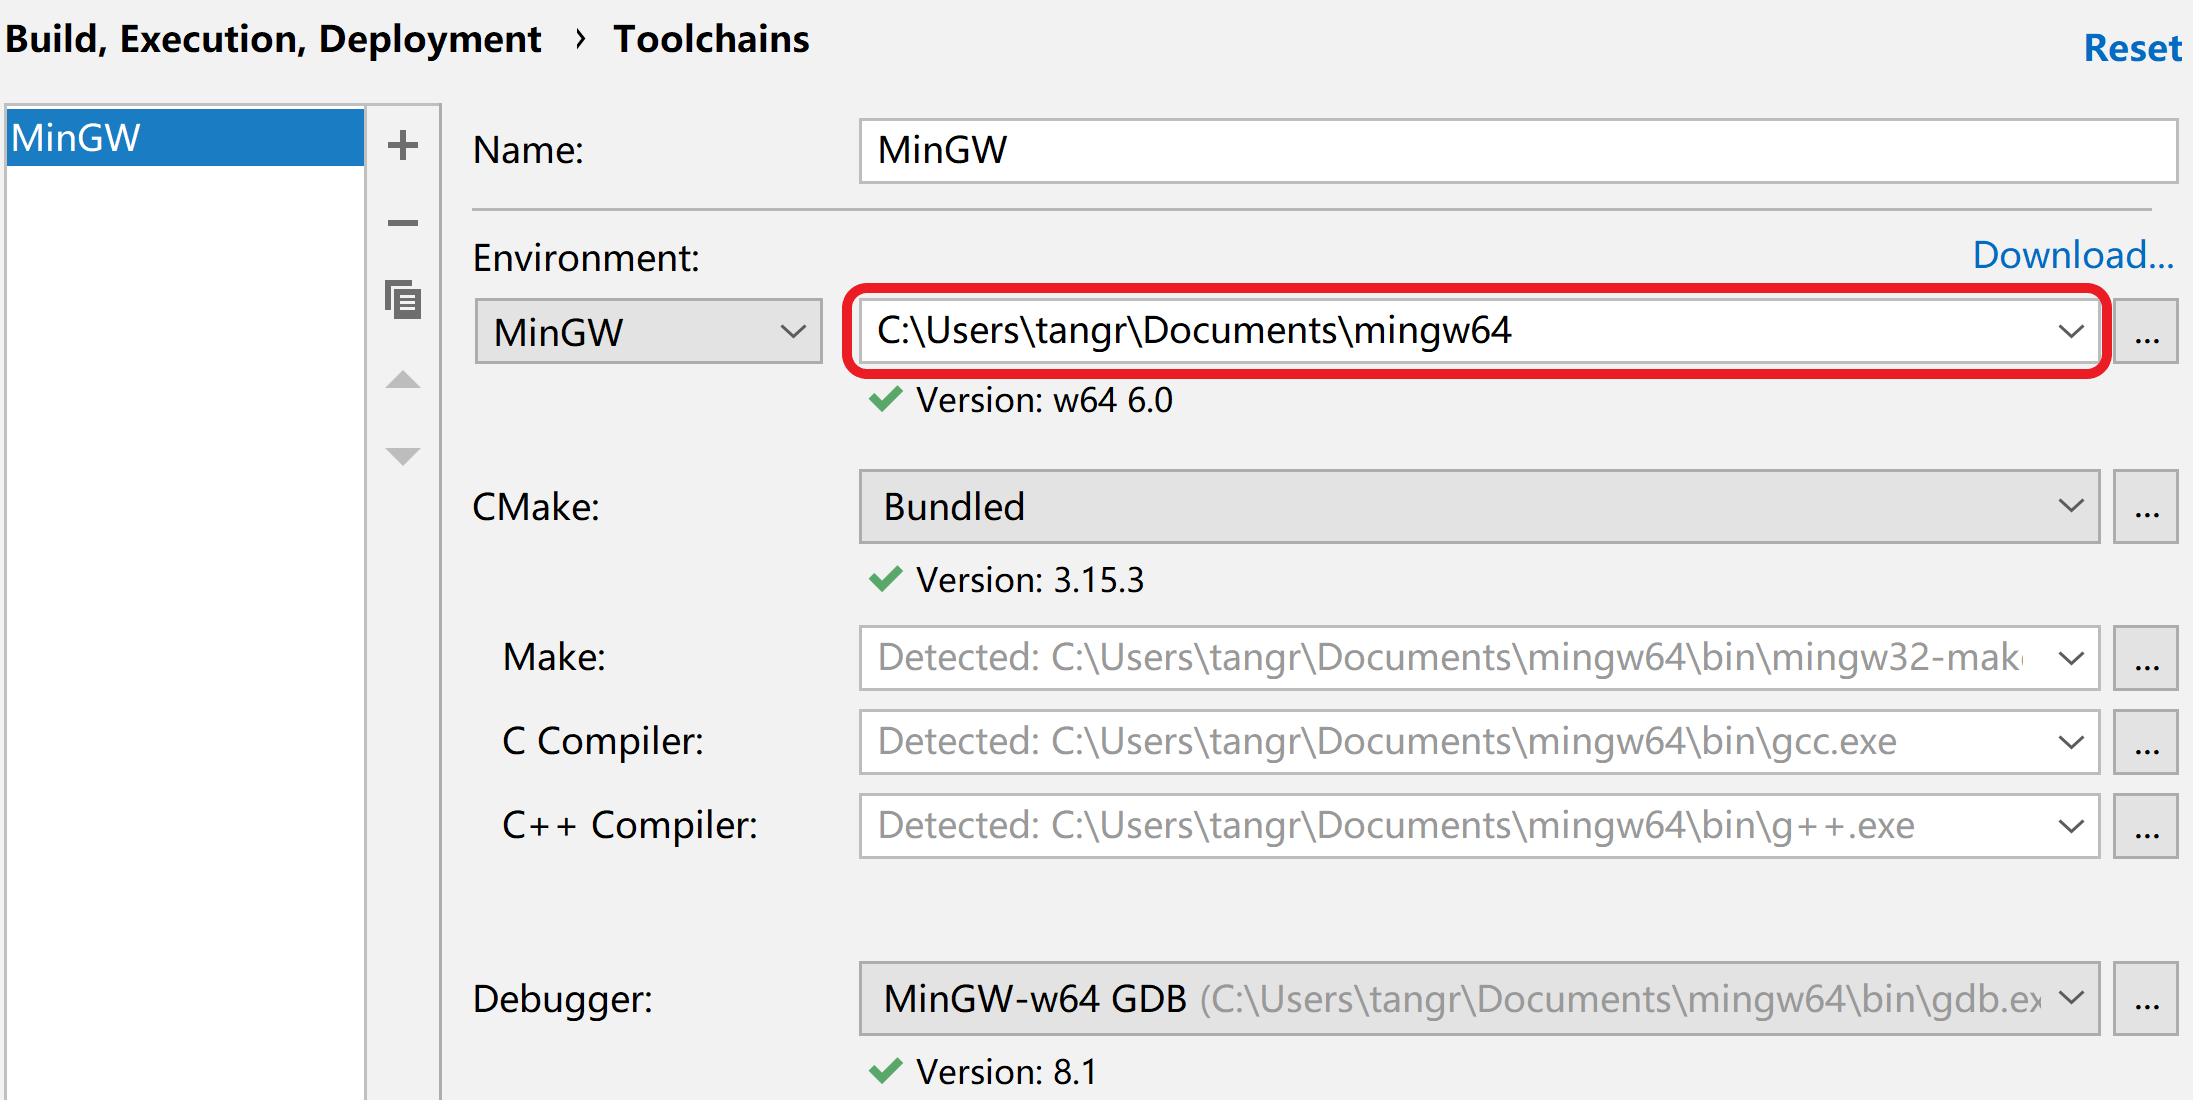
\includegraphics[width=75mm]{figs/clion_mingw.png}
\caption{CLion 配置MinGW}
\end{figure}
\end{frame}

\begin{frame}[fragile]{自定义 CMakeLists.txt}
下载 \href{http://problemoverflow.top/download/OJ.zip}{http://problemoverflow.top/download/OJ.zip}

解压并用CLion打开该目录, 打开 CMakeLists.txt

\emptyline

部分解释:
\begin{itemize}[<+- | alert@+>]

\item 第4-5行: 定义使用的标准为C99和C++11 (符合OJ设置)

\item 第7行: 使编译器产生更多警告, 并将警告视为错误 (比OJ严格)

\item 第8行: 定义了一个宏\texttt{DEBUG}, 用于 redirect.h (后面讲, 不影响OJ)

\item 第9行: math.h需要链接的数学函数库 (符合OJ设置)

\item 第11-22行: 定义多个可执行文件设置, 方便管理
\end{itemize}

\end{frame}


\begin{frame}[fragile]{输入输出重定向}
\begin{itemize}[<+- | alert@+>]
\item 调试OJ时, 一个很烦的事情是每次都需要重新输入

\item 程序员最讨厌重复劳动. 如何解决这个问题? 

\item 如果你用的是Linux, 一个很简单的方法就是输入重定向:
\begin{verbatim}
  ./sum <input.txt
  echo 1 2 3 | ./sum
\end{verbatim}

\item 但在用CLion的时候输入命令行仍然很麻烦
\item redirect.h 解决了这个问题
\begin{itemize}
\item 不提供输入文件时从命令行窗口读取用户输入
\item 提供输入文件时通过输入文件读取输入
\item 提供输出文件时输出到该文件
\end{itemize}
\end{itemize}
\end{frame}

\begin{frame}[fragile]{输入输出重定向}
\begin{itemize}[<+- | alert@+>]
\item 代码编写样例见 main.c
\item 命令行: \texttt{./main [input] [output]}  (中括号为可选)
\item 在Program arguments中添加 \texttt{../input/1-1-a\_sum.txt}
\emptyline\begin{figure}[ht!]
\centering
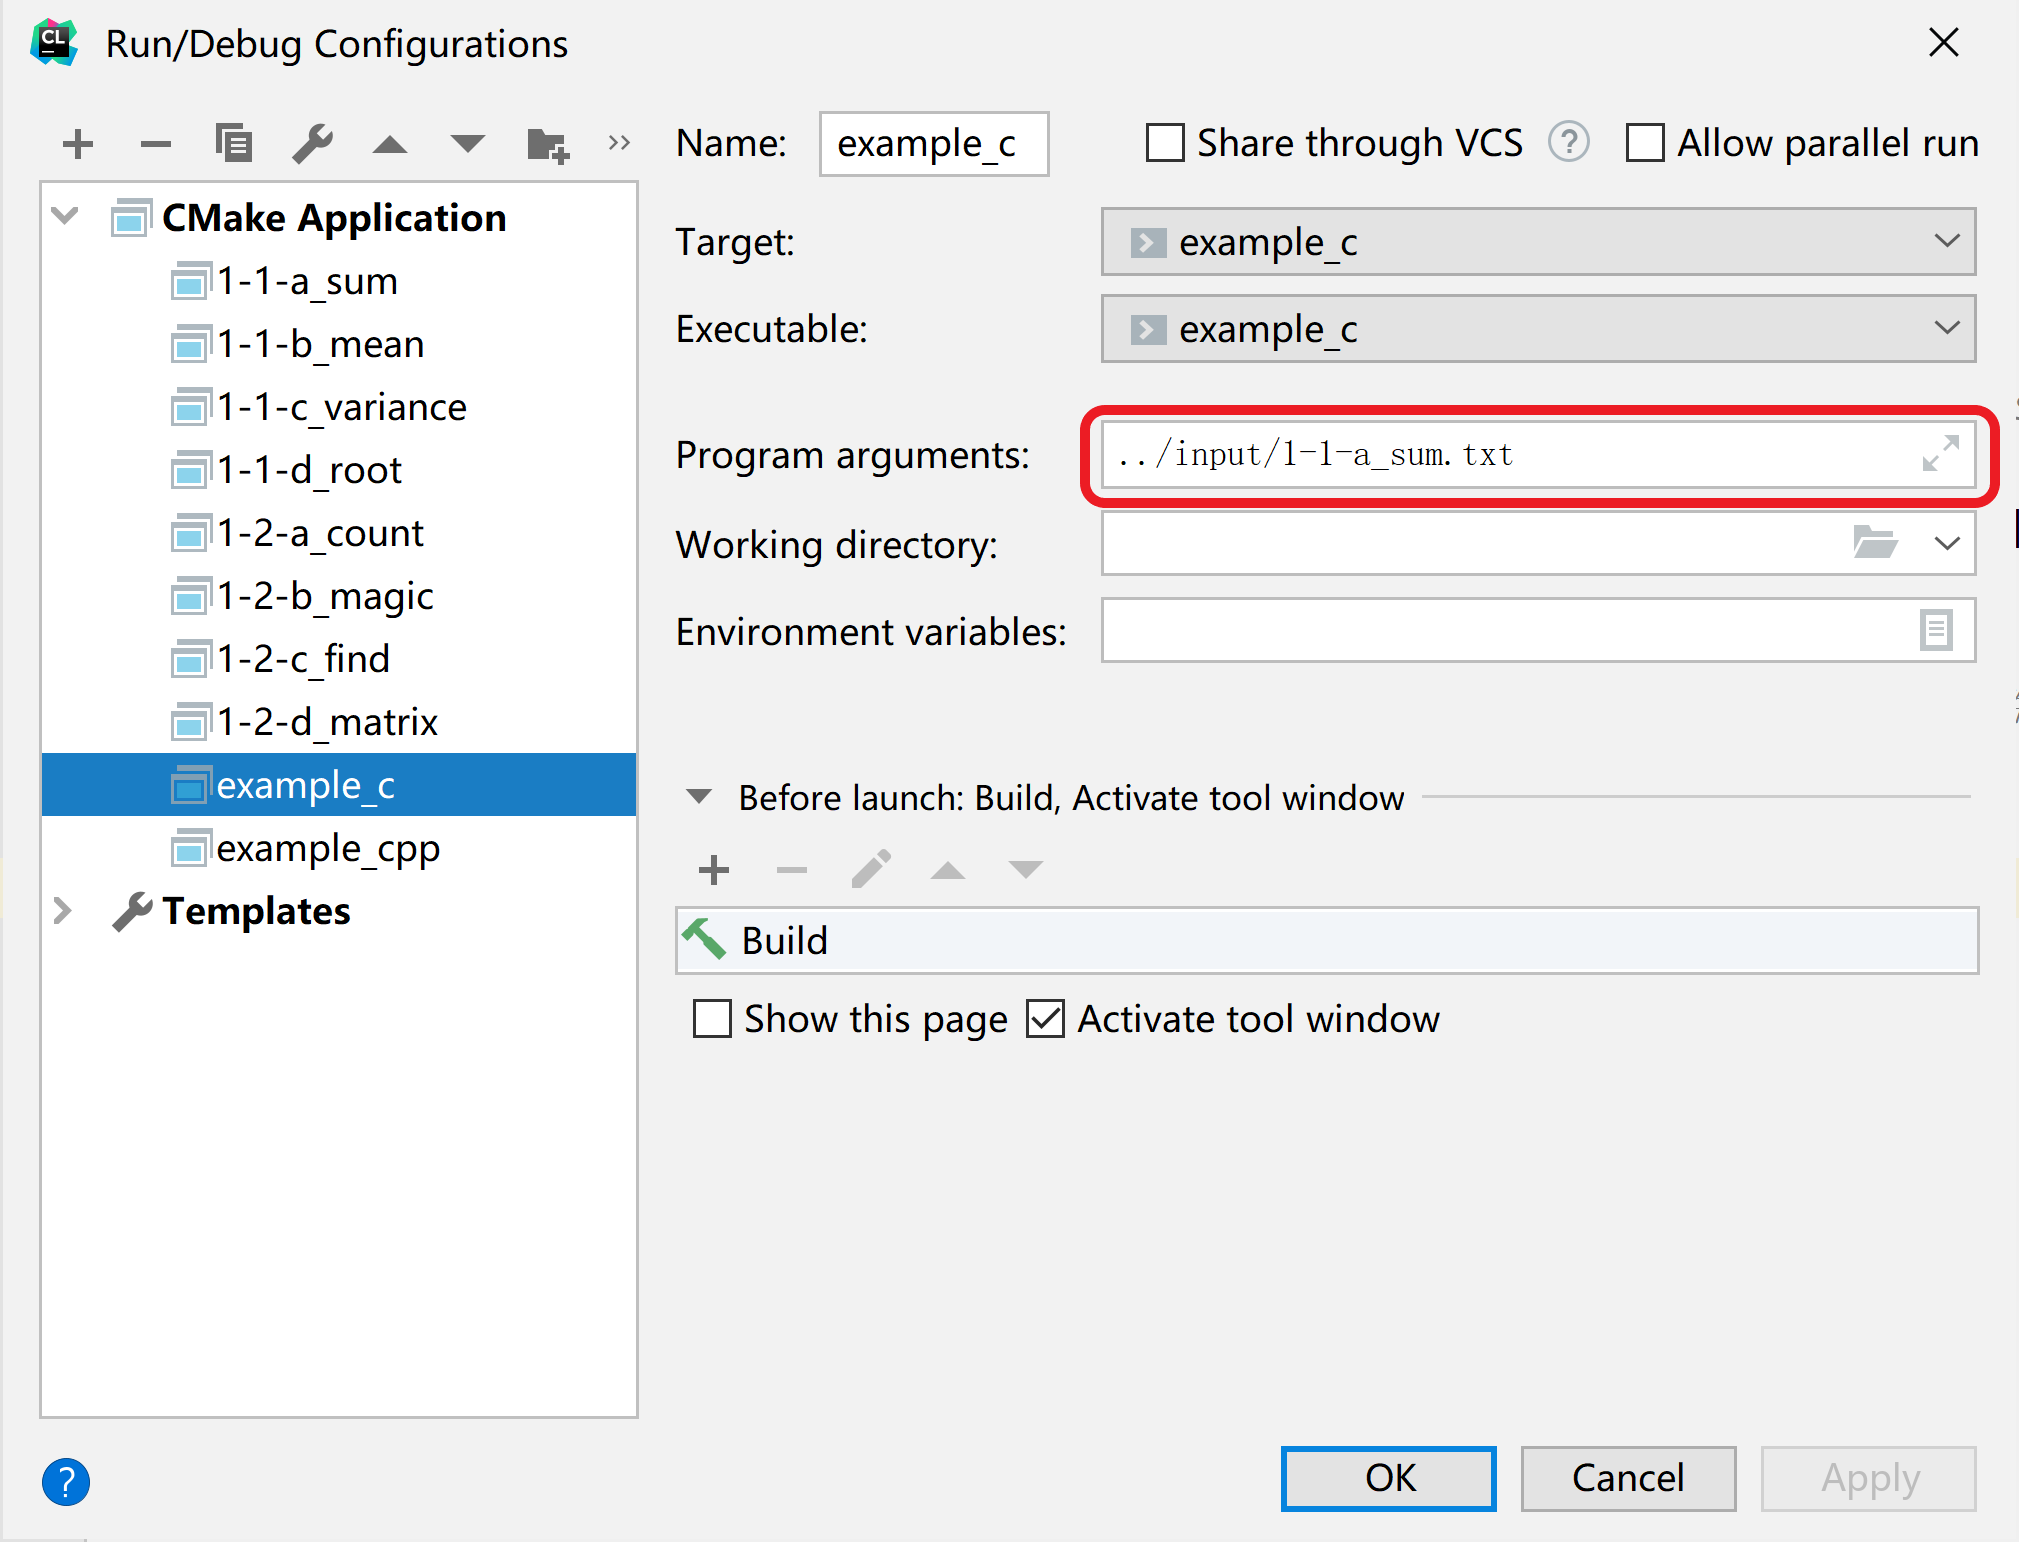
\includegraphics[width=65mm]{figs/clion_cmdargs.png}
\caption{CLion 添加命令行参数}
\end{figure}
\end{itemize}
\end{frame}


\section{C语言入门}

\begin{frame}[fragile]{再看第一个程序}
\begin{columns}[T,onlytextwidth]
\column{0.50\textwidth}
\emptyline
\emptyline
\emptyline
\small\begin{lstlisting}[language=c,numbers=left]
/* my first program in C */
#include <stdio.h>
int main() {
    printf("Hello, world!\n");
}
\end{lstlisting}

\column{0.05\textwidth}
\column{0.45\textwidth}
\begin{block}{第1行}
C语言风格注释, C99标准可以使用C++单行注释(//\ldots)
\end{block}
\begin{block}{第2行}
包含头文件, 该头文件声明了printf()函数(去掉编译试试?)
\end{block}
\begin{block}{第3行}
定义了main函数, 这个函数是程序入口(改个名字试试?)
\end{block}
\begin{block}{第4行}
输出\textquotedblleft \texttt{Hello, world!\textbackslash n}\textquotedblright
\end{block}
\end{columns}
\end{frame}

\begin{frame}[fragile]{变量}
\begin{verbatim}
int a = 8, b = 4, c = 7, d = 6, result_24;
result_24 = (a - c) * b * d;
\end{verbatim}
\begin{itemize}[<+- | alert@+>]
\item 代码中的\texttt{a}, \texttt{b}, \texttt{c}, \texttt{d}, \texttt{result\_24}是变量名
\item 变量名由字母, 数字和下划线(\_)组成
\item 不能以数字开头, 尽量不要以下划线开头
\item 不能是C语言关键词
\item \textbf{大小写敏感}
\end{itemize}
\end{frame}

\begin{frame}[fragile]{基本数据类型}
\begin{columns}[T,onlytextwidth]
\column{0.20\textwidth}
\begin{verbatim}
_Bool a;
char b;
int c;
double d;
\end{verbatim}

\column{0.80\textwidth}
\begin{itemize}[<+- | alert@+>]
\item 数据存储在内存中, 计算机看来都是01比特串
\item 变量名使计算机能找到变量存储在内存的什么地方
\item 而类型确定了该内存区域二进制值的转译方式
\item 代码中\texttt{bool}, \texttt{char}, \texttt{int}, \texttt{double}是几种数据类型
\item 具体解释见 \href{http://problemoverflow.top/c/1.C%E8%AF%AD%E8%A8%80%E5%85%A5%E9%97%A8/1.1.%E5%8F%98%E9%87%8F%E5%92%8C%E7%B1%BB%E5%9E%8B.html}{problemoverflow.top/c}
\item 可以编译运行main.cpp观察你的开发环境下各种数据类型的字节长度和最小值最大值
\end{itemize}
\end{columns}
\end{frame}

\begin{frame}[fragile]{条件语句}
\begin{itemize}[<+- | alert@+>]
\item 如果今天是周六, 我就出去玩; 如果是周日, 就睡大觉; 否则去上学 
\item 翻译成C代码:
\begin{verbatim}
if (today == SATURDAY) {
    // play outside
} else if (today == SUNDAY) {
    // sleep all day
} else {
    // go to school...
}
\end{verbatim}
\item if条件语句中的\texttt{else if}和\texttt{else}语句块不是必需的
\item 语句块中如果只有一个语句, 则可以去掉大括号
\item 相等(==), 不等(!=), 大于(>), 不小于(>=), 逻辑与(\&\&), 逻辑或(||)
\item \textbf{判断相等是两个等号}
\end{itemize}
\end{frame}

\begin{frame}[fragile]{循环语句}
\begin{quote}
Three or more, use a for.
\end{quote}

\begin{itemize}[<+- | alert@+>]
\item 程序员最讨厌重复劳动, 循环语句是消除重复劳动的利器
\item 现在让你打印 \texttt{Hello, world!} 三千遍
\item 我们分别用for循环和while循环实现:
\item \begin{verbatim}
for (int i = 0; i != 3000; ++i) {
    printf("Hello, world!\n");
}
\end{verbatim}
\item \begin{verbatim}
int i = 3000;
while (i--)
    printf("Hello, world!\n");
\end{verbatim}

\end{itemize}
\end{frame}

\begin{frame}[fragile]{格式化输出printf()}
\begin{itemize}[<+- | alert@+>]
\item 前面已经用过 printf() 了, 它的功能远不止打印 \texttt{Hello, world!}
\item 打印一个char类型字符ch: \texttt{printf("\%c", ch);}
\item 打印一个int类型的整数i: \texttt{printf("\%d", i);}
\item 打印一个short int类型的整数s: \texttt{printf("\%hd", s);}
\item 打印一个double类型的浮点数d和保留两位小数: \texttt{printf("\%f \%.2f", d, d);}
\item 观察有什么不同?
\end{itemize}
\end{frame}

\begin{frame}[fragile]{格式化输出printf()}
格式化字符串可以很复杂:
\href{http://www.cplusplus.com/reference/cstdio/printf/}{\texttt{\%[flags][width][.precision][length]\alert{specifier}}}
\begin{table}
\begin{tabular}{@{} cl @{}}
\toprule
\textbf{specifier} & \textbf{输出} \\
\midrule
d 或 i & 有符号十进制整数 \\
u & 无符号十进制整数 \\
o & 无符号八进制 \\
x & 无符号十六进制 \\
f & 十进制小数 \\
e & 科学计数法 \\
g & \%e或\%f输出长度短的 \\
c & 字符 \\
s & 字符串 \\
p & 指针地址 \\
\% & 打印特殊字符: \% \\
\bottomrule
\end{tabular}
\caption{常用的specifier}
\end{table}
\end{frame}

\begin{frame}[fragile]{格式化输出printf()}
\href{http://www.cplusplus.com/reference/cstdio/printf/}{\texttt{\%[flags][width][.precision]\alert{[length]}specifier}}
\begin{table}
\begin{tabular}{clll}
\toprule
 & \multicolumn{3}{c}{\textbf{specifiers}} \\
\textbf{length} & d i & u o x X & f F e E g G a A \\
\midrule
(none) & int & unsigned int & double \\
hh & signed char & unsigned char &  \\
h & short int & unsigned short int &  \\
l & long int & unsigned long int &  \\
ll & long long int & unsigned long long int & \\
\bottomrule
\end{tabular}
\caption{常用的length}
\end{table}
\end{frame}

\begin{frame}[fragile]{格式化输入scanf()}
\begin{itemize}[<+- | alert@+>]
\item 格式: \href{http://www.cplusplus.com/reference/cstdio/scanf/}{\%[*][width][length]specifier}
\item 读取整数到int类型变量i: \texttt{scanf("\%d", \alert{\&}i);}
\item 大多数specifier, length和printf()的相同
\item 除了double要用\texttt{\%lf}, 而 float 仍然用 \texttt{\%f}
\item printf()输出double也可以用 \texttt{\%lf}
\item 小技巧: scanf()的返回值表示成功读取了多少个变量, 如果小于等于0表示出错或者输入结束, 可以放在循环的条件中:
\begin{verbatim}
while (scanf("%d", &i) > 0)
    sum += i;
\end{verbatim}
\end{itemize}
\end{frame}

\begin{frame}[standout]
	Questions?
\end{frame}

\end{document}
